\chapter{The Vendetta}

At what point shall I begin my story, your excellency?” asked
Bertuccio.

“Where you please,” returned Monte Cristo, “since I know nothing at all
of it.”

“I thought the Abbé Busoni had told your excellency.”

“Some particulars, doubtless, but that is seven or eight years ago, and
I have forgotten them.”

“Then I can speak without fear of tiring your excellency.”

“Go on, M. Bertuccio; you will supply the want of the evening papers.”

“The story begins in 1815.”

“Ah,” said Monte Cristo, “1815 is not yesterday.”

“No, monsieur, and yet I recollect all things as clearly as if they had
happened but then. I had a brother, an elder brother, who was in the
service of the emperor; he had become lieutenant in a regiment composed
entirely of Corsicans. This brother was my only friend; we became
orphans—I at five, he at eighteen. He brought me up as if I had been
his son, and in 1814 he married. When the emperor returned from the
Island of Elba, my brother instantly joined the army, was slightly
wounded at Waterloo, and retired with the army beyond the Loire.”

“But that is the history of the Hundred Days, M. Bertuccio,” said the
count; “unless I am mistaken, it has been already written.”

“Excuse me, excellency, but these details are necessary, and you
promised to be patient.”

“Go on; I will keep my word.”

“One day we received a letter. I should tell you that we lived in the
little village of Rogliano, at the extremity of Cap Corse. This letter
was from my brother. He told us that the army was disbanded, and that
he should return by Châteauroux, Clermont-Ferrand, Le Puy, and Nîmes;
and, if I had any money, he prayed me to leave it for him at Nîmes,
with an innkeeper with whom I had dealings.”

“In the smuggling line?” said Monte Cristo.

“Eh, your excellency? Everyone must live.”

“Certainly; go on.”

“I loved my brother tenderly, as I told your excellency, and I resolved
not to send the money, but to take it to him myself. I possessed a
thousand francs. I left five hundred with Assunta, my sister-in-law,
and with the other five hundred I set off for Nîmes. It was easy to do
so, and as I had my boat and a lading to take in at sea, everything
favored my project. But, after we had taken in our cargo, the wind
became contrary, so that we were four or five days without being able
to enter the Rhône. At last, however, we succeeded, and worked up to
Arles. I left the boat between Bellegarde and Beaucaire, and took the
road to Nîmes.”

“We are getting to the story now?”

“Yes, your excellency; excuse me, but, as you will see, I only tell you
what is absolutely necessary. Just at this time the famous massacres
took place in the south of France. Three brigands, called Trestaillon,
Truphemy, and Graffan, publicly assassinated everybody whom they
suspected of Bonapartism. You have doubtless heard of these massacres,
your excellency?”

“Vaguely; I was far from France at that period. Go on.”

“As I entered Nîmes, I literally waded in blood; at every step you
encountered dead bodies and bands of murderers, who killed, plundered,
and burned. At the sight of this slaughter and devastation I became
terrified, not for myself—for I, a simple Corsican fisherman, had
nothing to fear; on the contrary, that time was most favorable for us
smugglers—but for my brother, a soldier of the empire, returning from
the army of the Loire, with his uniform and his epaulets, there was
everything to apprehend. I hastened to the innkeeper. My misgivings had
been but too true. My brother had arrived the previous evening at
Nîmes, and, at the very door of the house where he was about to demand
hospitality, he had been assassinated. I did all in my power to
discover the murderers, but no one durst tell me their names, so much
were they dreaded. I then thought of that French justice of which I had
heard so much, and which feared nothing, and I went to the king’s
attorney.”

“And this king’s attorney was named Villefort?” asked Monte Cristo
carelessly.

“Yes, your excellency; he came from Marseilles, where he had been
deputy procureur. His zeal had procured him advancement, and he was
said to be one of the first who had informed the government of the
departure from the Island of Elba.”

“Then,” said Monte Cristo “you went to him?”

“‘Monsieur,’ I said, ‘my brother was assassinated yesterday in the
streets of Nîmes, I know not by whom, but it is your duty to find out.
You are the representative of justice here, and it is for justice to
avenge those she has been unable to protect.’

“‘Who was your brother?’ asked he.

“‘A lieutenant in the Corsican battalion.’

“‘A soldier of the usurper, then?’

“‘A soldier of the French army.’

“‘Well,’ replied he, ‘he has smitten with the sword, and he has
perished by the sword.’

“‘You are mistaken, monsieur,’ I replied; ‘he has perished by the
poniard.’

“‘What do you want me to do?’ asked the magistrate.

“‘I have already told you—avenge him.’

“‘On whom?’

“‘On his murderers.’

“‘How should I know who they are?’

“‘Order them to be sought for.’

“‘Why, your brother has been involved in a quarrel, and killed in a
duel. All these old soldiers commit excesses which were tolerated in
the time of the emperor, but which are not suffered now, for the people
here do not like soldiers of such disorderly conduct.’

“‘Monsieur,’ I replied, ‘it is not for myself that I entreat your
interference—I should grieve for him or avenge him, but my poor brother
had a wife, and were anything to happen to me, the poor creature would
perish from want, for my brother’s pay alone kept her. Pray, try and
obtain a small government pension for her.’

“‘Every revolution has its catastrophes,’ returned M. de Villefort;
‘your brother has been the victim of this. It is a misfortune, and
government owes nothing to his family. If we are to judge by all the
vengeance that the followers of the usurper exercised on the partisans
of the king, when, in their turn, they were in power, your brother
would be today, in all probability, condemned to death. What has
happened is quite natural, and in conformity with the law of
reprisals.’

“‘What,’ cried I, ‘do you, a magistrate, speak thus to me?’

“‘All these Corsicans are mad, on my honor,’ replied M. de Villefort;
‘they fancy that their countryman is still emperor. You have mistaken
the time, you should have told me this two months ago, it is too late
now. Go now, at once, or I shall have you put out.’

“I looked at him an instant to see if there was anything to hope from
further entreaty. But he was a man of stone. I approached him, and said
in a low voice, ‘Well, since you know the Corsicans so well, you know
that they always keep their word. You think that it was a good deed to
kill my brother, who was a Bonapartist, because you are a royalist.
Well, I, who am a Bonapartist also, declare one thing to you, which is,
that I will kill you. From this moment I declare the vendetta against
you, so protect yourself as well as you can, for the next time we meet
your last hour has come.’ And before he had recovered from his
surprise, I opened the door and left the room.”

“Well, well,” said Monte Cristo, “such an innocent looking person as
you are to do those things, M. Bertuccio, and to a king’s attorney at
that! But did he know what was meant by the terrible word ‘vendetta’?”

“He knew so well, that from that moment he shut himself in his house,
and never went out unattended, seeking me high and low. Fortunately, I
was so well concealed that he could not find me. Then he became
alarmed, and dared not stay any longer at Nîmes, so he solicited a
change of residence, and, as he was in reality very influential, he was
nominated to Versailles. But, as you know, a Corsican who has sworn to
avenge himself cares not for distance, so his carriage, fast as it
went, was never above half a day’s journey before me, who followed him
on foot. The most important thing was, not to kill him only—for I had
an opportunity of doing so a hundred times—but to kill him without
being discovered—at least, without being arrested. I no longer belonged
to myself, for I had my sister-in-law to protect and provide for.

“For three months I watched M. de Villefort, for three months he took
not a step out-of-doors without my following him. At length I
discovered that he went mysteriously to Auteuil. I followed him
thither, and I saw him enter the house where we now are, only, instead
of entering by the great door that looks into the street, he came on
horseback, or in his carriage, left the one or the other at the little
inn, and entered by the gate you see there.”

Monte Cristo made a sign with his head to show that he could discern in
the darkness the door to which Bertuccio alluded.

“As I had nothing more to do at Versailles, I went to Auteuil, and
gained all the information I could. If I wished to surprise him, it was
evident this was the spot to lie in wait for him. The house belonged,
as the concierge informed your excellency, to M. de Saint-Méran,
Villefort’s father-in-law. M. de Saint-Méran lived at Marseilles, so
that this country house was useless to him, and it was reported to be
let to a young widow, known only by the name of ‘the Baroness.’

“One evening, as I was looking over the wall, I saw a young and
handsome woman who was walking alone in that garden, which was not
overlooked by any windows, and I guessed that she was awaiting M. de
Villefort. When she was sufficiently near for me to distinguish her
features, I saw she was from eighteen to nineteen, tall and very fair.
As she had a loose muslin dress on and as nothing concealed her figure,
I saw she would ere long become a mother. A few moments after, the
little door was opened and a man entered. The young woman hastened to
meet him. They threw themselves into each other’s arms, embraced
tenderly, and returned together to the house. The man was M. de
Villefort; I fully believed that when he went out in the night he would
be forced to traverse the whole of the garden alone.”

\begin{figure}[h]
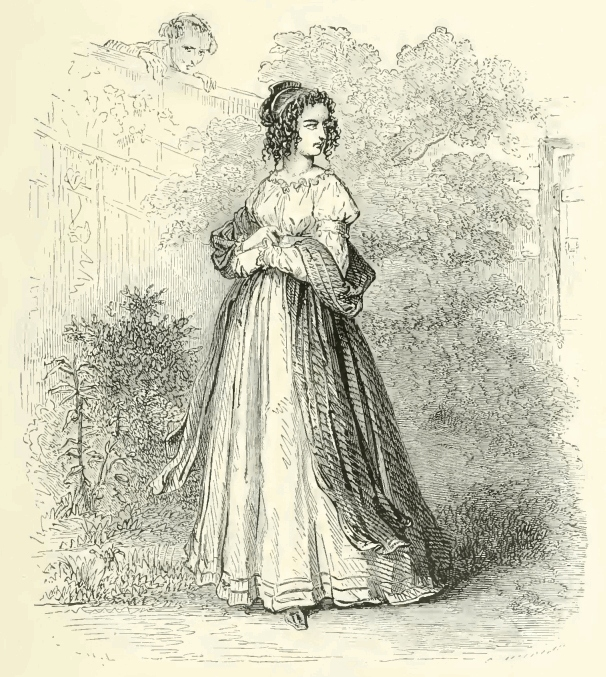
\includegraphics[width=\textwidth]{20291m.jpg}
\end{figure}

“And,” asked the count, “did you ever know the name of this woman?”

“No, excellency,” returned Bertuccio; “you will see that I had no time
to learn it.”

“Go on.”

“That evening,” continued Bertuccio, “I could have killed the
procureur, but as I was not sufficiently acquainted with the
neighborhood, I was fearful of not killing him on the spot, and that if
his cries were overheard I might be taken; so I put it off until the
next occasion, and in order that nothing should escape me, I took a
chamber looking into the street bordered by the wall of the garden.
Three days after, about seven o’clock in the evening, I saw a servant
on horseback leave the house at full gallop, and take the road to
Sèvres. I concluded that he was going to Versailles, and I was not
deceived. Three hours later, the man returned covered with dust, his
errand was performed, and two minutes after, another man on foot,
muffled in a mantle, opened the little door of the garden, which he
closed after him. I descended rapidly; although I had not seen
Villefort’s face, I recognized him by the beating of my heart. I
crossed the street, and stopped at a post placed at the angle of the
wall, and by means of which I had once before looked into the garden.

“This time I did not content myself with looking, but I took my knife
out of my pocket, felt that the point was sharp, and sprang over the
wall. My first care was to run to the door; he had left the key in it,
taking the simple precaution of turning it twice in the lock. Nothing,
then, preventing my escape by this means, I examined the grounds. The
garden was long and narrow; a stretch of smooth turf extended down the
middle, and at the corners were clumps of trees with thick and massy
foliage, that made a background for the shrubs and flowers. In order to
go from the door to the house, or from the house to the door, M. de
Villefort would be obliged to pass by one of these clumps of trees.

\begin{figure}[ht]
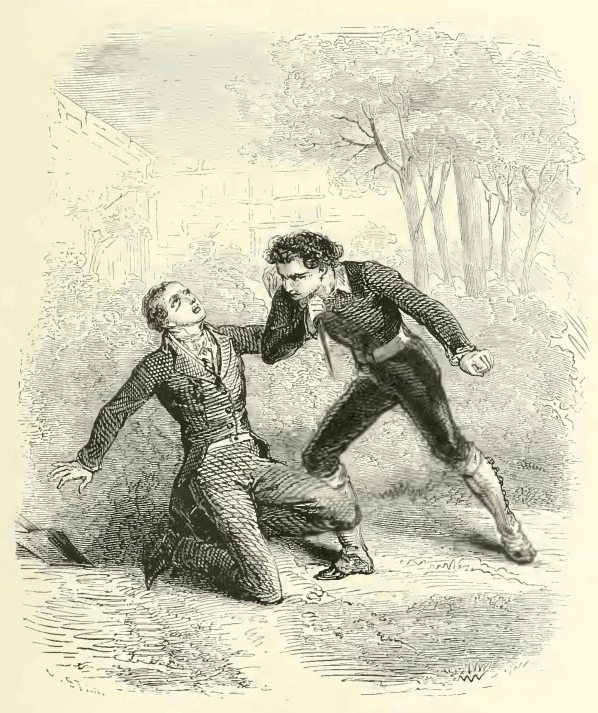
\includegraphics[width=\textwidth]{20293m.jpg}
\end{figure}

“It was the end of September; the wind blew violently. The faint
glimpses of the pale moon, hidden momentarily by masses of dark clouds
that were sweeping across the sky, whitened the gravel walks that led
to the house, but were unable to pierce the obscurity of the thick
shrubberies, in which a man could conceal himself without any fear of
discovery. I hid myself in the one nearest to the path Villefort must
take, and scarcely was I there when, amidst the gusts of wind, I
fancied I heard groans; but you know, or rather you do not know, your
excellency, that he who is about to commit an assassination fancies
that he hears low cries perpetually ringing in his ears. Two hours
passed thus, during which I imagined I heard moans repeatedly. Midnight
struck. As the last stroke died away, I saw a faint light shine through
the windows of the private staircase by which we have just descended.
The door opened, and the man in the mantle reappeared.

“The terrible moment had come, but I had so long been prepared for it
that my heart did not fail in the least. I drew my knife from my pocket
again, opened it, and made ready to strike. The man in the mantle
advanced towards me, but as he drew near I saw that he had a weapon in
his hand. I was afraid, not of a struggle, but of a failure. When he
was only a few paces from me, I saw that what I had taken for a weapon
was only a spade. I was still unable to divine for what reason M. de
Villefort had this spade in his hands, when he stopped close to the
thicket where I was, glanced round, and began to dig a hole in the
earth. I then perceived that he was hiding something under his mantle,
which he laid on the grass in order to dig more freely. Then, I
confess, curiosity mingled with hatred; I wished to see what Villefort
was going to do there, and I remained motionless, holding my breath.
Then an idea crossed my mind, which was confirmed when I saw the
procureur lift from under his mantle a box, two feet long, and six or
eight inches deep. I let him place the box in the hole he had made,
then, while he stamped with his feet to remove all traces of his
occupation, I rushed on him and plunged my knife into his breast,
exclaiming:

“‘I am Giovanni Bertuccio; thy death for my brother’s; thy treasure for
his widow; thou seest that my vengeance is more complete than I had
hoped.’

“I know not if he heard these words; I think he did not, for he fell
without a cry. I felt his blood gush over my face, but I was
intoxicated, I was delirious, and the blood refreshed, instead of
burning me. In a second I had disinterred the box; then, that it might
not be known I had done so, I filled up the hole, threw the spade over
the wall, and rushed through the door, which I double-locked, carrying
off the key.”

“Ah,” said Monte Cristo “it seems to me this was nothing but murder and
robbery.”

“No, your excellency,” returned Bertuccio; “it was a vendetta followed
by restitution.”

“And was the sum a large one?”

“It was not money.”

“Ah, I recollect,” replied the count; “did you not say something of an
infant?”

“Yes, excellency; I hastened to the river, sat down on the bank, and
with my knife forced open the lock of the box. In a fine linen cloth
was wrapped a new-born child. Its purple visage, and its violet-colored
hands showed that it had perished from suffocation, but as it was not
yet cold, I hesitated to throw it into the water that ran at my feet.
After a moment I fancied that I felt a slight pulsation of the heart,
and as I had been assistant at the hospital at Bastia, I did what a
doctor would have done—I inflated the lungs by blowing air into them,
and at the expiration of a quarter of an hour, it began to breathe, and
cried feebly. In my turn I uttered a cry, but a cry of joy.

“‘God has not cursed me then,’ I cried, ‘since he permits me to save
the life of a human creature, in exchange for the life I have taken
away.’”

\begin{figure}[ht]
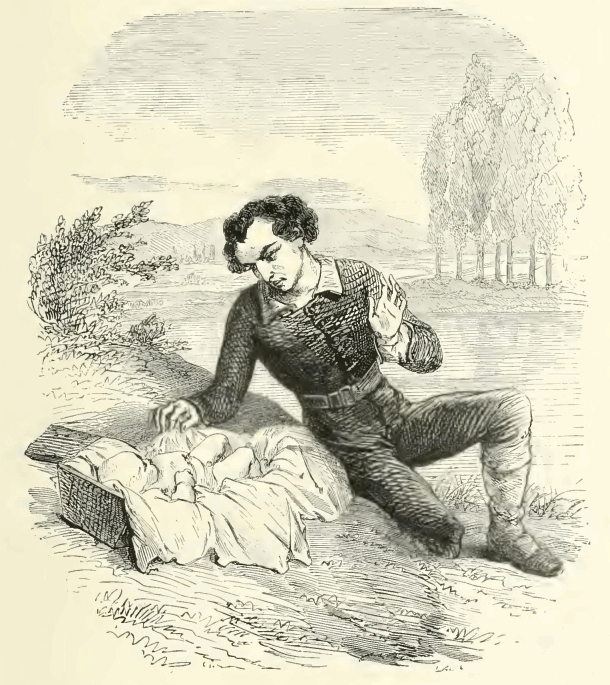
\includegraphics[width=\textwidth]{20295m.jpg}
\end{figure}

“And what did you do with the child?” asked Monte Cristo. “It was an
embarrassing load for a man seeking to escape.”

“I had not for a moment the idea of keeping it, but I knew that at
Paris there was an asylum where they receive such creatures. As I
passed the city gates I declared that I had found the child on the
road, and I inquired where the asylum was; the box confirmed my
statement, the linen proved that the infant belonged to wealthy
parents, the blood with which I was covered might have proceeded from
the child as well as from anyone else. No objection was raised, but
they pointed out the asylum, which was situated at the upper end of the
Rue d’Enfer, and after having taken the precaution of cutting the linen
in two pieces, so that one of the two letters which marked it was on
the piece wrapped around the child, while the other remained in my
possession, I rang the bell, and fled with all speed. A fortnight after
I was at Rogliano, and I said to Assunta:

“‘Console thyself, sister; Israel is dead, but he is avenged.’

“She demanded what I meant, and when I had told her all,—‘Giovanni,’
said she, ‘you should have brought this child with you; we would have
replaced the parents it has lost, have called it Benedetto, and then,
in consequence of this good action, God would have blessed us.’ In
reply I gave her the half of the linen I had kept in order to reclaim
him if we became rich.”

“What letters were marked on the linen?” said Monte Cristo.

“An H and an N, surmounted by a baron’s coronet.”

“By heaven, M. Bertuccio, you make use of heraldic terms; where did you
study heraldry?”

“In your service, excellency, where everything is learned.”

“Go on, I am curious to know two things.”

“What are they, your excellency?”

“What became of this little boy? for I think you told me it was a boy,
M. Bertuccio.”

“No excellency, I do not recollect telling you that.”

“I thought you did; I must have been mistaken.”

“No, you were not, for it was in reality a little boy. But your
excellency wished to know two things; what was the second?”

“The second was the crime of which you were accused when you asked for
a confessor, and the Abbé Busoni came to visit you at your request in
the prison at Nîmes.”

“The story will be very long, excellency.”

“What matter? you know I take but little sleep, and I do not suppose
you are very much inclined for it either.” Bertuccio bowed, and resumed
his story.

“Partly to drown the recollections of the past that haunted me, partly
to supply the wants of the poor widow, I eagerly returned to my trade
of smuggler, which had become more easy since that relaxation of the
laws which always follows a revolution. The southern districts were
ill-watched in particular, in consequence of the disturbances that were
perpetually breaking out in Avignon, Nîmes, or Uzès. We profited by
this respite on the part of the government to make friends everywhere.
Since my brother’s assassination in the streets of Nîmes, I had never
entered the town; the result was that the innkeeper with whom we were
connected, seeing that we would no longer come to him, was forced to
come to us, and had established a branch to his inn, on the road from
Bellegarde to Beaucaire, at the sign of the Pont du Gard. We had thus,
at Aigues-Mortes, Martigues, or Bouc, a dozen places where we left our
goods, and where, in case of necessity, we concealed ourselves from the
gendarmes and custom-house officers. Smuggling is a profitable trade,
when a certain degree of vigor and intelligence is employed; as for
myself, brought up in the mountains, I had a double motive for fearing
the gendarmes and custom-house officers, as my appearance before the
judges would cause an inquiry, and an inquiry always looks back into
the past. And in my past life they might find something far more grave
than the selling of smuggled cigars, or barrels of brandy without a
permit. So, preferring death to capture, I accomplished the most
astonishing deeds, and which, more than once, showed me that the too
great care we take of our bodies is the only obstacle to the success of
those projects which require rapid decision, and vigorous and
determined execution. In reality, when you have once devoted your life
to your enterprises, you are no longer the equal of other men, or,
rather, other men are no longer your equals, and whosoever has taken
this resolution, feels his strength and resources doubled.”

“Philosophy, M. Bertuccio,” interrupted the count; “you have done a
little of everything in your life.”

“Oh, excellency!”

“No, no; but philosophy at half-past ten at night is somewhat late; yet
I have no other observation to make, for what you say is correct, which
is more than can be said for all philosophy.”

“My journeys became more and more extensive and more productive.
Assunta took care of all, and our little fortune increased. One day as
I was setting off on an expedition, ‘Go,’ said she; ‘at your return I
will give you a surprise.’ I questioned her, but in vain; she would
tell me nothing, and I departed. Our expedition lasted nearly six
weeks; we had been to Lucca to take in oil, to Leghorn for English
cottons, and we ran our cargo without opposition, and returned home
full of joy. When I entered the house, the first thing I beheld in the
middle of Assunta’s chamber was a cradle that might be called sumptuous
compared with the rest of the furniture, and in it a baby seven or
eight months old. I uttered a cry of joy; the only moments of sadness I
had known since the assassination of the procureur were caused by the
recollection that I had abandoned this child. For the assassination
itself I had never felt any remorse. Poor Assunta had guessed all. She
had profited by my absence, and furnished with the half of the linen,
and having written down the day and hour at which I had deposited the
child at the asylum, had set off for Paris, and had reclaimed it. No
objection was raised, and the infant was given up to her. Ah, I
confess, your excellency, when I saw this poor creature sleeping
peacefully in its cradle, I felt my eyes filled with tears. ‘Ah,
Assunta,’ cried I, ‘you are an excellent woman, and Heaven will bless
you.’”

“This,” said Monte Cristo, “is less correct than your philosophy,—it is
only faith.”

“Alas, your excellency is right,” replied Bertuccio, “and God made this
infant the instrument of our punishment. Never did a perverse nature
declare itself more prematurely, and yet it was not owing to any fault
in his bringing up. He was a most lovely child, with large blue eyes,
of that deep color that harmonizes so well with the blond complexion;
only his hair, which was too light, gave his face a most singular
expression, and added to the vivacity of his look, and the malice of
his smile.

“Unfortunately, there is a proverb which says that ‘red is either
altogether good or altogether bad.’ The proverb was but too correct as
regarded Benedetto, and even in his infancy he manifested the worst
disposition. It is true that the indulgence of his foster-mother
encouraged him. This child, for whom my poor sister would go to the
town, five or six leagues off, to purchase the earliest fruits and the
most tempting sweetmeats, preferred to Palma grapes or Genoese
preserves, the chestnuts stolen from a neighbor’s orchard, or the dried
apples in his loft, when he could eat as well of the nuts and apples
that grew in my garden.

“One day, when Benedetto was about five or six, our neighbor Wasilio,
who, according to the custom of the country, never locked up his purse
or his valuables—for, as your excellency knows, there are no thieves in
Corsica—complained that he had lost a louis out of his purse; we
thought he must have made a mistake in counting his money, but he
persisted in the accuracy of his statement. One day, Benedetto, who had
been gone from the house since morning, to our great anxiety, did not
return until late in the evening, dragging a monkey after him, which he
said he had found chained to the foot of a tree. For more than a month
past, the mischievous child, who knew not what to wish for, had taken
it into his head to have a monkey. A boatman, who had passed by
Rogliano, and who had several of these animals, whose tricks had
greatly diverted him, had, doubtless, suggested this idea to him.
‘Monkeys are not found in our woods chained to trees,’ said I; ‘confess
how you obtained this animal.’ Benedetto maintained the truth of what
he had said, and accompanied it with details that did more honor to his
imagination than to his veracity. I became angry; he began to laugh, I
threatened to strike him, and he made two steps backwards. ‘You cannot
beat me,’ said he; ‘you have no right, for you are not my father.’

\begin{figure}[ht]
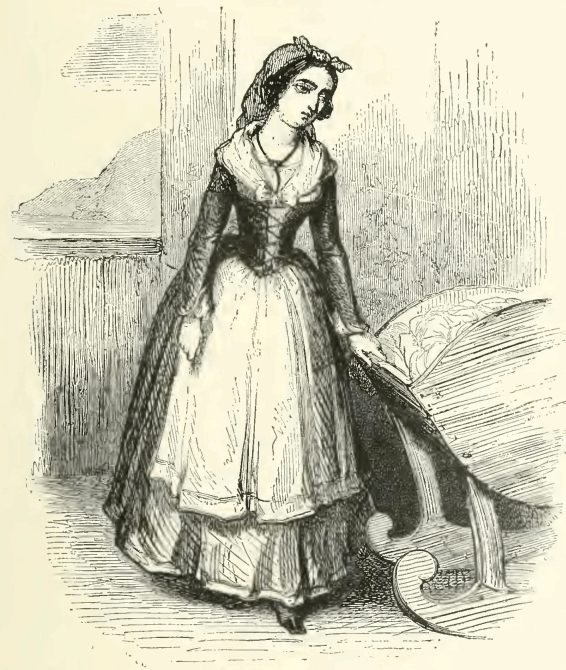
\includegraphics[width=\textwidth]{20299m.jpg}
\end{figure}

“We never knew who had revealed this fatal secret, which we had so
carefully concealed from him; however, it was this answer, in which the
child’s whole character revealed itself, that almost terrified me, and
my arm fell without touching him.

“The boy triumphed, and this victory rendered him so audacious, that
all the money of Assunta, whose affection for him seemed to increase as
he became more unworthy of it, was spent in caprices she knew not how
to contend against, and follies she had not the courage to prevent.
When I was at Rogliano everything went on properly, but no sooner was
my back turned than Benedetto became master, and everything went ill.
When he was only eleven, he chose his companions from among the young
men of eighteen or twenty, the worst characters in Bastia, or, indeed,
in Corsica, and they had already, for some mischievous pranks, been
several times threatened with a prosecution. I became alarmed, as any
prosecution might be attended with serious consequences. I was
compelled, at this period, to leave Corsica on an important expedition;
I reflected for a long time, and with the hope of averting some
impending misfortune, I resolved that Benedetto should accompany me.

“I hoped that the active and laborious life of a smuggler, with the
severe discipline on board, would have a salutary effect on his
character, which was now well-nigh, if not quite, corrupt. I spoke to
Benedetto alone, and proposed to him to accompany me, endeavoring to
tempt him by all the promises most likely to dazzle the imagination of
a child of twelve. He heard me patiently, and when I had finished,
burst out laughing.

“‘Are you mad, uncle?’ (he called me by this name when he was in good
humor); ‘do you think I am going to change the life I lead for your
mode of existence—my agreeable indolence for the hard and precarious
toil you impose on yourself, exposed to the bitter frost at night, and
the scorching heat by day, compelled to conceal yourself, and when you
are perceived, receive a volley of bullets, all to earn a paltry sum?
Why, I have as much money as I want; mother Assunta always furnishes me
when I ask for it! You see that I should be a fool to accept your
offer.’

“The arguments, and his audacity, perfectly stupefied me. Benedetto
rejoined his associates, and I saw him from a distance point me out to
them as a fool.”

“Sweet child,” murmured Monte Cristo.

“Oh, had he been my own son,” replied Bertuccio, “or even my nephew, I
would have brought him back to the right road, for the knowledge that
you are doing your duty gives you strength, but the idea that I was
striking a child whose father I had killed, made it impossible for me
to punish him. I gave my sister, who constantly defended the
unfortunate boy, good advice, and as she confessed that she had several
times missed money to a considerable amount, I showed her a safe place
in which to conceal our little treasure for the future. My mind was
already made up. Benedetto could read, write, and cipher perfectly, for
when the fit seized him, he learned more in a day than others in a
week. My intention was to enter him as a clerk in some ship, and
without letting him know anything of my plan, to convey him some
morning on board; by this means his future treatment would depend upon
his own conduct. I set off for France, after having fixed upon the
plan. Our cargo was to be landed in the Gulf of Lyons, and this was a
difficult thing to do because it was then the year 1829. The most
perfect tranquillity was restored, and the vigilance of the
custom-house officers was redoubled, and their strictness was increased
at this time, in consequence of the fair at Beaucaire.

\begin{figure}[h]
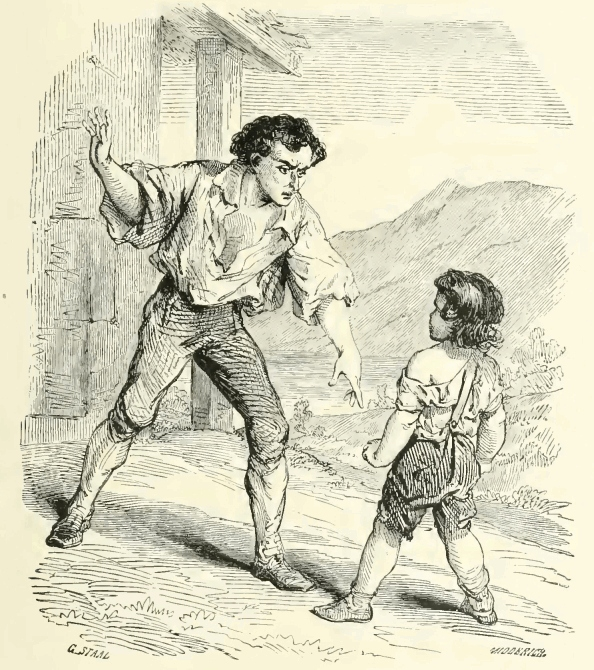
\includegraphics[width=\textwidth]{20301m.jpg}
\end{figure}

“Our expedition made a favorable beginning. We anchored our
vessel—which had a double hold, where our goods were concealed—amidst a
number of other vessels that bordered the banks of the Rhône from
Beaucaire to Arles. On our arrival we began to discharge our cargo in
the night, and to convey it into the town, by the help of the innkeeper
with whom we were connected.

“Whether success rendered us imprudent, or whether we were betrayed, I
know not; but one evening, about five o’clock, our little cabin-boy
came breathlessly, to inform us that he had seen a detachment of
custom-house officers advancing in our direction. It was not their
proximity that alarmed us, for detachments were constantly patrolling
along the banks of the Rhône, but the care, according to the boy’s
account, that they took to avoid being seen. In an instant we were on
the alert, but it was too late; our vessel was surrounded, and amongst
the custom-house officers I observed several gendarmes, and, as
terrified at the sight of their uniforms as I was brave at the sight of
any other, I sprang into the hold, opened a port, and dropped into the
river, dived, and only rose at intervals to breathe, until I reached a
ditch that had recently been made from the Rhône to the canal that runs
from Beaucaire to Aigues-Mortes. I was now safe, for I could swim along
the ditch without being seen, and I reached the canal in safety. I had
designedly taken this direction. I have already told your excellency of
an innkeeper from Nîmes who had set up a little tavern on the road from
Bellegarde to Beaucaire.”

“Yes,” said Monte Cristo “I perfectly recollect him; I think he was
your colleague.”

“Precisely,” answered Bertuccio; “but he had, seven or eight years
before this period, sold his establishment to a tailor at Marseilles,
who, having almost ruined himself in his old trade, wished to make his
fortune in another. Of course, we made the same arrangements with the
new landlord that we had with the old; and it was of this man that I
intended to ask shelter.”

“What was his name?” inquired the count, who seemed to become somewhat
interested in Bertuccio’s story.

“Gaspard Caderousse; he had married a woman from the village of
Carconte, and whom we did not know by any other name than that of her
village. She was suffering from malarial fever, and seemed dying by
inches. As for her husband, he was a strapping fellow of forty, or
five-and-forty, who had more than once, in time of danger, given ample
proof of his presence of mind and courage.”

“And you say,” interrupted Monte Cristo “that this took place towards
the year——”

“1829, your excellency.”

“In what month?”

“June.”

“The beginning or the end?”

“The evening of the 3rd.”

\begin{figure}[ht]
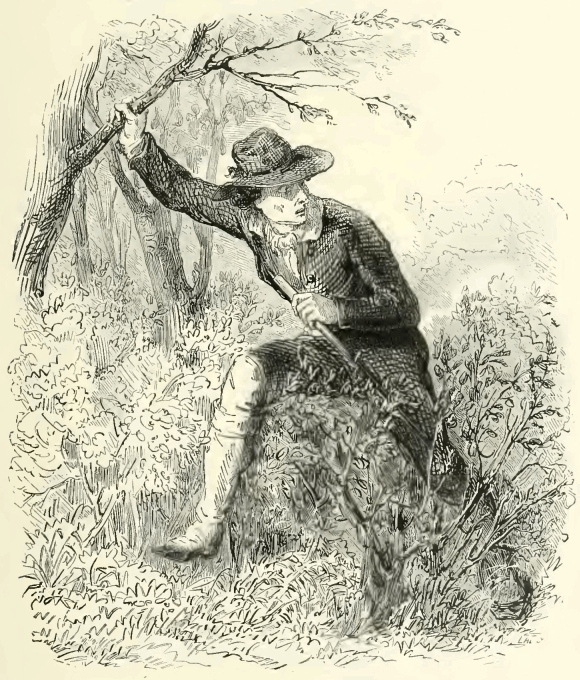
\includegraphics[width=\textwidth]{20303m.jpg}
\end{figure}

“Ah,” said Monte Cristo “the evening of the 3rd of June, 1829. Go on.”

“It was from Caderousse that I intended demanding shelter, and, as we
never entered by the door that opened onto the road, I resolved not to
break through the rule, so climbing over the garden-hedge, I crept
amongst the olive and wild fig trees, and fearing that Caderousse might
have some guest, I entered a kind of shed in which I had often passed
the night, and which was only separated from the inn by a partition, in
which holes had been made in order to enable us to watch an opportunity
of announcing our presence.

“My intention was, if Caderousse was alone, to acquaint him with my
presence, finish the meal the custom-house officers had interrupted,
and profit by the threatened storm to return to the Rhône, and
ascertain the state of our vessel and its crew. I stepped into the
shed, and it was fortunate I did so, for at that moment Caderousse
entered with a stranger.

“I waited patiently, not to overhear what they said, but because I
could do nothing else; besides, the same thing had occurred often
before. The man who was with Caderousse was evidently a stranger to the
South of France; he was one of those merchants who come to sell
jewellery at the Beaucaire fair, and who during the month the fair
lasts, and during which there is so great an influx of merchants and
customers from all parts of Europe, often have dealings to the amount
of 100,000 to 150,000 francs. Caderousse entered hastily. Then, seeing
that the room was, as usual, empty, and only guarded by the dog, he
called to his wife, ‘Hello, Carconte,’ said he, ‘the worthy priest has
not deceived us; the diamond is real.’

“An exclamation of joy was heard, and the staircase creaked beneath a
feeble step. ‘What do you say?’ asked his wife, pale as death.

“‘I say that the diamond is real, and that this gentleman, one of the
first jewellers of Paris, will give us 50,000 francs for it. Only, in
order to satisfy himself that it really belongs to us, he wishes you to
relate to him, as I have done already, the miraculous manner in which
the diamond came into our possession. In the meantime please to sit
down, monsieur, and I will fetch you some refreshment.’

“The jeweller examined attentively the interior of the inn and the
apparent poverty of the persons who were about to sell him a diamond
that seemed to have come from the casket of a prince.

“‘Relate your story, madame,’ said he, wishing, no doubt, to profit by
the absence of the husband, so that the latter could not influence the
wife’s story, to see if the two recitals tallied.

“‘Oh,’ returned she, ‘it was a gift of heaven. My husband was a great
friend, in 1814 or 1815, of a sailor named Edmond Dantès. This poor
fellow, whom Caderousse had forgotten, had not forgotten him, and at
his death he bequeathed this diamond to him.’

“‘But how did he obtain it?’ asked the jeweller; ‘had he it before he
was imprisoned?’

“‘No, monsieur; but it appears that in prison he made the acquaintance
of a rich Englishman, and as in prison he fell sick, and Dantès took
the same care of him as if he had been his brother, the Englishman,
when he was set free, gave this stone to Dantès, who, less fortunate,
died, and, in his turn, left it to us, and charged the excellent abbé,
who was here this morning, to deliver it.’

“‘The same story,’ muttered the jeweller; ‘and improbable as it seemed
at first, it may be true. There’s only the price we are not agreed
about.’

“‘How not agreed about?’ said Caderousse. ‘I thought we agreed for the
price I asked.’

“‘That is,’ replied the jeweller, ‘I offered 40,000 francs.’

‘Forty thousand,’ cried La Carconte; ‘we will not part with it for that
sum. The abbé told us it was worth 50,000 without the setting.’

“‘What was the abbé’s name?’ asked the indefatigable questioner.

“‘The Abbé Busoni,’ said La Carconte.

“‘He was a foreigner?’

“‘An Italian from the neighborhood of Mantua, I believe.’

“‘Let me see this diamond again,’ replied the jeweller; ‘the first time
you are often mistaken as to the value of a stone.’

“Caderousse took from his pocket a small case of black shagreen,
opened, and gave it to the jeweller. At the sight of the diamond, which
was as large as a hazel-nut, La Carconte’s eyes sparkled with
cupidity.”

“And what did you think of this fine story, eavesdropper?” said Monte
Cristo; “did you credit it?”

“Yes, your excellency. I did not look on Caderousse as a bad man, and I
thought him incapable of committing a crime, or even a theft.”

“That did more honor to your heart than to your experience, M.
Bertuccio. Had you known this Edmond Dantès, of whom they spoke?”

“No, your excellency, I had never heard of him before, and never but
once afterwards, and that was from the Abbé Busoni himself, when I saw
him in the prison at Nîmes.”

“Go on.”

“The jeweller took the ring, and drawing from his pocket a pair of
steel pliers and a small set of copper scales, he took the stone out of
its setting, and weighed it carefully.

“‘I will give you 45,000,’ said he, ‘but not a sou more; besides, as
that is the exact value of the stone, I brought just that sum with me.’

“‘Oh, that’s no matter,’ replied Caderousse, ‘I will go back with you
to fetch the other 5,000 francs.’

“‘No,’ returned the jeweller, giving back the diamond and the ring to
Caderousse, ‘no, it is worth no more, and I am sorry I offered so much,
for the stone has a flaw in it, which I had not seen. However, I will
not go back on my word, and I will give 45,000.’

“‘At least, replace the diamond in the ring,’ said La Carconte sharply.

“‘Ah, true,’ replied the jeweller, and he reset the stone.

“‘No matter,’ observed Caderousse, replacing the box in his pocket,
‘someone else will purchase it.’

“‘Yes,’ continued the jeweller; ‘but someone else will not be so easy
as I am, or content himself with the same story. It is not natural that
a man like you should possess such a diamond. He will inform against
you. You will have to find the Abbé Busoni; and abbés who give diamonds
worth two thousand louis are rare. The law would seize it, and put you
in prison; if at the end of three or four months you are set at
liberty, the ring will be lost, or a false stone, worth three francs,
will be given you, instead of a diamond worth 50,000 or perhaps 55,000
francs; from which you must allow that one runs considerable risk in
purchasing.’

“Caderousse and his wife looked eagerly at each other.

“‘No,’ said Caderousse, ‘we are not rich enough to lose 5,000 francs.’

“‘As you please, my dear sir,’ said the jeweller; ‘I had, however, as
you see, brought you the money in bright coin.’ And he drew from his
pocket a handful of gold, and held it sparkling before the dazzled eyes
of the innkeeper, and in the other hand he held a packet of bank-notes.

“There was evidently a severe struggle in the mind of Caderousse; it
was plain that the small shagreen case, which he turned over and over
in his hand, did not seem to him commensurate in value to the enormous
sum which fascinated his gaze. He turned towards his wife.

“‘What do you think of this?’ he asked in a low voice.

“‘Let him have it—let him have it,’ she said. ‘If he returns to
Beaucaire without the diamond, he will inform against us, and, as he
says, who knows if we shall ever again see the Abbé Busoni?—in all
probability we shall never see him.’

“‘Well, then, so I will!’ said Caderousse; ‘so you may have the diamond
for 45,000 francs. But my wife wants a gold chain, and I want a pair of
silver buckles.’

“The jeweller drew from his pocket a long flat box, which contained
several samples of the articles demanded. ‘Here,’ he said, ‘I am very
straightforward in my dealings—take your choice.’

“The woman selected a gold chain worth about five louis, and the
husband a pair of buckles, worth perhaps fifteen francs.

“‘I hope you will not complain now?’ said the jeweller.

“‘The abbé told me it was worth 50,000 francs,’ muttered Caderousse.

“‘Come, come—give it to me! What a strange fellow you are,’ said the
jeweller, taking the diamond from his hand. ‘I give you 45,000
francs—that is, 2,500 livres of income,—a fortune such as I wish I had
myself, and you are not satisfied!’

“‘And the five-and-forty thousand francs,’ inquired Caderousse in a
hoarse voice, ‘where are they? Come—let us see them.’

“‘Here they are,’ replied the jeweller, and he counted out upon the
table 15,000 francs in gold, and 30,000 francs in bank-notes.

“‘Wait whilst I light the lamp,’ said La Carconte; ‘it is growing dark,
and there may be some mistake.’ In fact, night had come on during this
conversation, and with night the storm which had been threatening for
the last half-hour. The thunder growled in the distance; but it was
apparently not heard by the jeweller, Caderousse, or La Carconte,
absorbed as they were all three with the demon of gain. I myself felt
a strange kind of fascination at the sight of all this gold and all
these bank-notes; it seemed to me that I was in a dream, and, as it
always happens in a dream, I felt myself riveted to the spot.
Caderousse counted and again counted the gold and the notes, then
handed them to his wife, who counted and counted them again in her
turn. During this time, the jeweller made the diamond play and sparkle
in the lamplight, and the gem threw out jets of light which made him
unmindful of those which—precursors of the storm—began to play in at
the windows.

“‘Well,’ inquired the jeweller, ‘is the cash all right?’

“‘Yes,’ said Caderousse. ‘Give me the pocket-book, La Carconte, and
find a bag somewhere.’

“La Carconte went to a cupboard, and returned with an old leathern
pocket-book and a bag. From the former she took some greasy letters,
and put in their place the bank-notes, and from the bag took two or
three crowns of six livres each, which, in all probability, formed the
entire fortune of the miserable couple.

“‘There,’ said Caderousse; ‘and now, although you have wronged us of
perhaps 10,000 francs, will you have your supper with us? I invite you
with good-will.’

“‘Thank you,’ replied the jeweller, ‘it must be getting late, and I
must return to Beaucaire—my wife will be getting uneasy.’ He drew out
his watch, and exclaimed, ‘\textit{Morbleu!} nearly nine o’clock—why, I shall
not get back to Beaucaire before midnight! Good-night, my friends. If
the Abbé Busoni should by any accident return, think of me.’

“‘In another week you will have left Beaucaire,’ remarked Caderousse,
‘for the fair ends in a few days.’

“‘True, but that makes no difference. Write to me at Paris, to M.
Joannes, in the Palais Royal, arcade Pierre, No. 45. I will make the
journey on purpose to see him, if it is worth while.’

“At this moment there was a tremendous clap of thunder, accompanied by
a flash of lightning so vivid, that it quite eclipsed the light of the
lamp.

\begin{figure}[h]
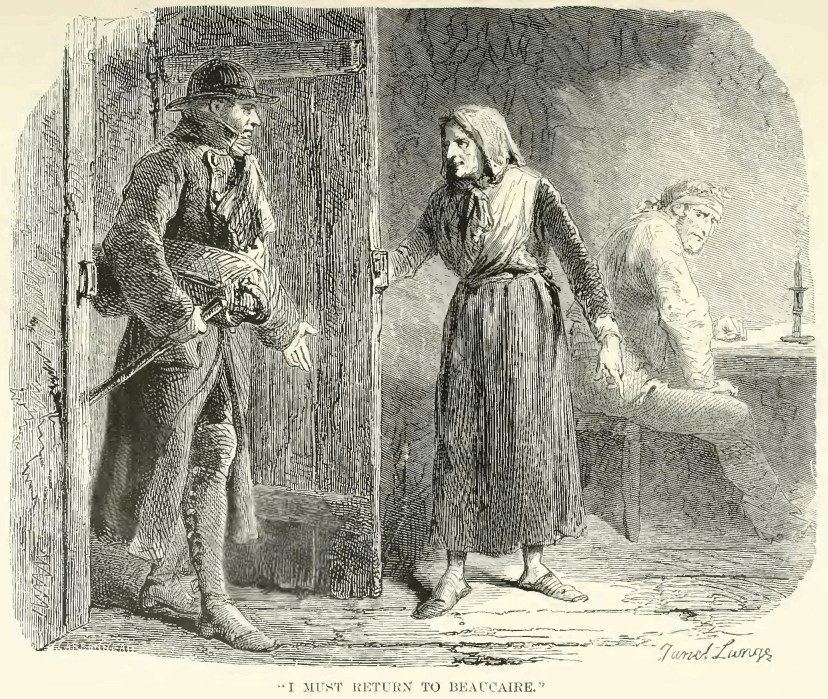
\includegraphics[width=\textwidth]{20307m.jpg}
\end{figure}

“‘See here,’ exclaimed Caderousse. ‘You cannot think of going out in
such weather as this.’

“‘Oh, I am not afraid of thunder,’ said the jeweller.

“‘And then there are robbers,’ said La Carconte. ‘The road is never
very safe during fair time.’

“‘Oh, as to the robbers,’ said Joannes, ‘here is something for them,’
and he drew from his pocket a pair of small pistols, loaded to the
muzzle. ‘Here,’ said he, ‘are dogs who bark and bite at the same time,
they are for the two first who shall have a longing for your diamond,
Friend Caderousse.’

“Caderousse and his wife again interchanged a meaning look. It seemed
as though they were both inspired at the same time with some horrible
thought. ‘Well, then, a good journey to you,’ said Caderousse.

“‘Thanks,’ replied the jeweller. He then took his cane, which he had
placed against an old cupboard, and went out. At the moment when he
opened the door, such a gust of wind came in that the lamp was nearly
extinguished. ‘Oh,’ said he, ‘this is very nice weather, and two
leagues to go in such a storm.’

“‘Remain,’ said Caderousse. ‘You can sleep here.’

“‘Yes; do stay,’ added La Carconte in a tremulous voice; ‘we will take
every care of you.’

“‘No; I must sleep at Beaucaire. So, once more, good-night.’ Caderousse
followed him slowly to the threshold. ‘I can see neither heaven nor
earth,’ said the jeweller, who was outside the door. ‘Do I turn to the
right, or to the left hand?’

“‘To the right,’ said Caderousse. ‘You cannot go wrong—the road is
bordered by trees on both sides.’

“‘Good—all right,’ said a voice almost lost in the distance.

“‘Close the door,’ said La Carconte; ‘I do not like open doors when it
thunders.’

“‘Particularly when there is money in the house, eh?’ answered
Caderousse, double-locking the door.

\begin{figure}[h]
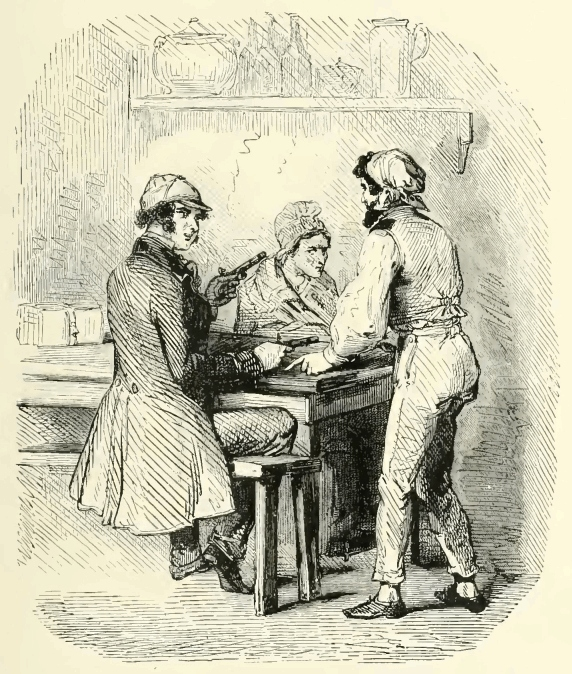
\includegraphics[width=\textwidth]{20311m.jpg}
\end{figure}

“He came into the room, went to the cupboard, took out the bag and
pocket-book, and both began, for the third time, to count their gold
and bank-notes. I never saw such an expression of cupidity as the
flickering lamp revealed in those two countenances. The woman,
especially, was hideous; her usual feverish tremulousness was
intensified, her countenance had become livid, and her eyes resembled
burning coals.

“‘Why,’ she inquired in a hoarse voice, ‘did you invite him to sleep
here tonight?’

“‘Why?’ said Caderousse with a shudder; ‘why, that he might not have
the trouble of returning to Beaucaire.’

“‘Ah,’ responded the woman, with an expression impossible to describe;
‘I thought it was for something else.’

“‘Woman, woman—why do you have such ideas?’ cried Caderousse; ‘or, if
you have them, why don’t you keep them to yourself?’

“‘Well,’ said La Carconte, after a moment’s pause, ‘you are not a man.’

“‘What do you mean?’ added Caderousse.

“‘If you had been a man, you would not have let him go from here.’

“‘Woman!’

“‘Or else he should not have reached Beaucaire.’

“‘Woman!’

“‘The road takes a turn—he is obliged to follow it—while alongside of
the canal there is a shorter road.’

“‘Woman!—you offend the good God. There—listen!’

And at this moment there was a tremendous peal of thunder, while the
livid lightning illumined the room, and the thunder, rolling away in
the distance, seemed to withdraw unwillingly from the cursed abode.
‘Mercy!’ said Caderousse, crossing himself.

\begin{figure}[ht]
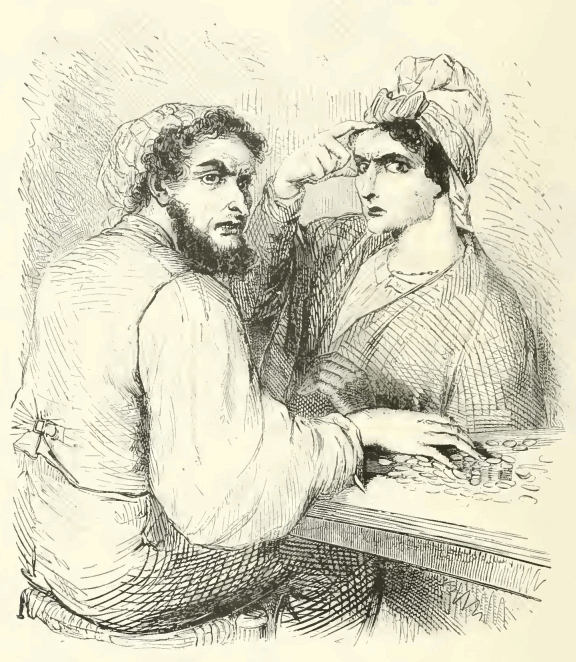
\includegraphics[width=\textwidth]{20312m.jpg}
\end{figure}

“At the same moment, and in the midst of the terrifying silence which
usually follows a clap of thunder, they heard a knocking at the door.
Caderousse and his wife started and looked aghast at each other.

“‘Who’s there?’ cried Caderousse, rising, and drawing up in a heap the
gold and notes scattered over the table, and which he covered with his
two hands.

“‘It is I,’ shouted a voice.

“‘And who are you?’

“‘Eh, \textit{pardieu!} Joannes, the jeweller.’

“‘Well, and you said I offended the good God,’ said La Carconte with a
horrid smile. ‘Why, the good God sends him back again.’ Caderousse sank
pale and breathless into his chair.

“La Carconte, on the contrary, rose, and going with a firm step towards
the door, opened it, saying, as she did so:

“‘Come in, dear M. Joannes.’

“‘\textit{Ma foi},’ said the jeweller, drenched with rain, ‘I am not destined
to return to Beaucaire tonight. The shortest follies are best, my dear
Caderousse. You offered me hospitality, and I accept it, and have
returned to sleep beneath your friendly roof.’

“Caderousse stammered out something, while he wiped away the sweat that
started to his brow. La Carconte double-locked the door behind the
jeweller.”
